\documentclass[tikz,border=14pt]{standalone}
\usepackage[T1]{fontenc}
\usepackage{tgheros}
\usepackage{sfmath}
\usepackage{amsmath}
\usepackage{fontawesome5}
\usepackage{tikz}
\usetikzlibrary{arrows.meta,positioning,shapes.geometric,fit,backgrounds,calc}
\usepackage{xcolor}

\renewcommand{\familydefault}{\sfdefault}

% Harvard Crimson & ETH Zurich Academic Semantic Palette
\definecolor{harvardcrimson}{HTML}{A51C30}
\definecolor{ethdarkblue}{HTML}{1F407A}
\definecolor{ethblue}{HTML}{215CAF}
\definecolor{ethpetrol}{HTML}{007A87}
\definecolor{ethbronze}{HTML}{B87333}
\definecolor{ethpurple}{HTML}{5B4B8A}
\definecolor{ethslate}{HTML}{475569}
\definecolor{cardbg}{HTML}{F8FAFC}
\definecolor{cardborder}{HTML}{CBD5E1}
\definecolor{safeTeal}{HTML}{10B981}

\begin{document}
\begin{tikzpicture}[
  font=\sffamily,
  >=Stealth,
  claimnode/.style={
    draw=harvardcrimson,
    fill=harvardcrimson!10,
    rounded corners=5pt,
    line width=1.3pt,
    text width=9.20in,
    inner sep=8pt,
    align=center
  },
  argnode/.style={
    draw=ethblue,
    fill=ethblue!8,
    rounded corners=4pt,
    line width=1pt,
    text width=2.10in,
    minimum height=1.20in,
    inner sep=6pt,
    align=left,
    anchor=north
  },
  evidencenode/.style={
    draw=safeTeal,
    fill=safeTeal!8,
    rounded corners=3pt,
    line width=0.8pt,
    text width=2.10in,
    minimum height=1.35in,
    inner sep=5pt,
    align=left,
    anchor=north
  },
  verdictnode/.style={
    draw=ethdarkblue,
    fill=white,
    rounded corners=5pt,
    line width=1.2pt,
    text width=9.20in,
    inner sep=7pt,
    align=center
  }
]

  % Top Title Banner
  \node[draw=ethdarkblue, fill=ethdarkblue!5, rounded corners=5pt, line width=1pt, text width=10.00in, inner sep=7pt, align=center] (title) at (5.00in, 0) {
    {\normalsize\bfseries\color{ethdarkblue}\faIcon{sitemap}\;\; CLAIM-ARGUMENT-EVIDENCE (CAE) SAFETY CASE ARCHITECTURE}\\[2pt]
    {\scriptsize\color{ethslate}Linking High-Level Safety Claims to Defensible Bench Metrology and Signed Release Verdicts}
  };

  % Top Level Claim
  \node[claimnode, below=0.20in of title] (c_top) {
    {\small\bfseries\color{harvardcrimson}\faIcon{bullseye}\; TOP-LEVEL SAFETY CLAIM ($C_{\text{top}}$)}\\[2pt]
    {\footnotesize\bfseries "The Physical AI Agent operates acceptably safe within Operational Design Domain $\mathcal{X}_{\text{ODD}}$."}
  };

  % --- 4 ARGUMENT NODES ---
  \node[argnode] (a1) at (1.10in, -1.80in) {
    {\scriptsize\bfseries\color{ethblue}\faIcon{shield-alt}\; ARGUMENT $A_1$}\\[2pt]
    {\tiny\bfseries Fault Containment}\\[4pt]
    {\tiny\color{ethslate}All single-point hardware and software crashes are \mbox{deterministically} arrested by the MCU safety enforcer within $50\text{ ms}$.}
  };

  \node[argnode] (a2) at (3.70in, -1.80in) {
    {\scriptsize\bfseries\color{ethblue}\faIcon{tachometer-alt}\; ARGUMENT $A_2$}\\[2pt]
    {\tiny\bfseries Latency Freshness}\\[4pt]
    {\tiny\color{ethslate}The $P_{99.9}$ sense-to-actuation latency $\Delta t_{\text{wall}}$ remains strictly bounded so stopping distance $d_{\text{stop}} \le d_{\text{gap}}$.}
  };

  \node[argnode] (a3) at (6.30in, -1.80in) {
    {\scriptsize\bfseries\color{ethblue}\faIcon{user-shield}\; ARGUMENT $A_3$}\\[2pt]
    {\tiny\bfseries Human Authority}\\[4pt]
    {\tiny\color{ethslate}Human operators retain un-preemptible authority via \mbox{bumpless} joystick override and dedicated hardware E-stop circuits.}
  };

  \node[argnode] (a4) at (8.90in, -1.80in) {
    {\scriptsize\bfseries\color{ethblue}\faIcon{compass}\; ARGUMENT $A_4$}\\[2pt]
    {\tiny\bfseries ODD Enforcement}\\[4pt]
    {\tiny\color{ethslate}Real-time interoceptive and exteroceptive health monitors detect out-of-ODD transitions and trigger safe deceleration.}
  };

  % --- 4 EVIDENCE NODES ---
  \node[evidencenode] (e1) at (1.10in, -3.25in) {
    {\scriptsize\bfseries\color{safeTeal}\faIcon{file-medical-alt}\; EVIDENCE $E_1$}\\[2pt]
    {\tiny\bfseries HIL Fault Log (\texttt{REL-01})}\\[4pt]
    {\tiny\color{ethslate}
    $\bullet$ $1000/1000$ faults contained\\
    $\bullet$ 0 collisions recorded\\
    $\bullet$ Max stopping time: $42\text{ ms}$\\
    $\bullet$ Watchdog trip: $50\text{ ms}$
    }
  };

  \node[evidencenode] (e2) at (3.70in, -3.25in) {
    {\scriptsize\bfseries\color{safeTeal}\faIcon{chart-line}\; EVIDENCE $E_2$}\\[2pt]
    {\tiny\bfseries Metrology CDF (\texttt{REQ-01})}\\[4pt]
    {\tiny\color{ethslate}
    $\bullet$ $P_{50} = 22\text{ ms}$\\
    $\bullet$ $P_{99.9} = 72\text{ ms} < 80\text{ ms}$\\
    $\bullet$ Margin: $+18\text{ cm}$ \mbox{clearance}\\
    $\bullet$ Zero seqlock overruns
    }
  };

  \node[evidencenode] (e3) at (6.30in, -3.25in) {
    {\scriptsize\bfseries\color{safeTeal}\faIcon{gamepad}\; EVIDENCE $E_3$}\\[2pt]
    {\tiny\bfseries Override Logs (\texttt{AUTH-01})}\\[4pt]
    {\tiny\color{ethslate}
    $\bullet$ $50/50$ seamless takeovers\\
    $\bullet$ Peak jerk $< 15\text{ rad/s}^3$\\
    $\bullet$ Zero gearbox shock damage\\
    $\bullet$ Tamper-evident hash log
    }
  };

  \node[evidencenode] (e4) at (8.90in, -3.25in) {
    {\scriptsize\bfseries\color{safeTeal}\faIcon{cloud-sun}\; EVIDENCE $E_4$}\\[2pt]
    {\tiny\bfseries ODD Monitor Logs}\\[4pt]
    {\tiny\color{ethslate}
    $\bullet$ Dark/glare detection $< 20\text{ ms}$\\
    $\bullet$ Friction drop fallback\\
    $\bullet$ Thermal derating at $85^\circ\text{C}$\\
    $\bullet$ Category 1 stop verified
    }
  };

  % Connecting Lines: Claim -> Arguments
  \draw[->, line width=1.1pt, harvardcrimson] (c_top.south) -- (a1.north);
  \draw[->, line width=1.1pt, harvardcrimson] (c_top.south) -- (a2.north);
  \draw[->, line width=1.1pt, harvardcrimson] (c_top.south) -- (a3.north);
  \draw[->, line width=1.1pt, harvardcrimson] (c_top.south) -- (a4.north);

  % Connecting Lines: Arguments -> Evidence
  \draw[->, line width=1.1pt, ethblue] (a1.south) -- (e1.north);
  \draw[->, line width=1.1pt, ethblue] (a2.south) -- (e2.north);
  \draw[->, line width=1.1pt, ethblue] (a3.south) -- (e3.north);
  \draw[->, line width=1.1pt, ethblue] (a4.south) -- (e4.north);

  % Bottom Release Verdict Node
  \node[verdictnode, below=0.20in of e2.south, anchor=north] (verdict) at (5.00in, -4.85in) {
    {\small\bfseries\color{ethdarkblue}\faIcon{signature}\;\; THE 3 ACCOUNTABLE RELEASE VERDICTS}\\[3pt]
    {\scriptsize
    \textbf{\color{safeTeal}\faIcon{check-circle}\; DEPLOY} (All evidence thresholds met; unconstrained ODD) \quad$\vert$\quad
    \textbf{\color{ethbronze}\faIcon{exclamation-circle}\; CONDITION} (Restricted speed / active human supervisor) \quad$\vert$\quad
    \textbf{\color{harvardcrimson}\faIcon{times-circle}\; REFUSE} (Gate failure; deployment blocked)
    }
  };

  \draw[->, line width=1.1pt, safeTeal] (e1.south) -- (e1.south |- verdict.north);
  \draw[->, line width=1.1pt, safeTeal] (e2.south) -- (verdict.north);
  \draw[->, line width=1.1pt, safeTeal] (e3.south) -- (verdict.north);
  \draw[->, line width=1.1pt, safeTeal] (e4.south) -- (e4.south |- verdict.north);

\end{tikzpicture}
\end{document}
